\begin{enumerate}[label=\thesection.\arabic*,ref=\thesection.\theenumi]
  \item Find the equation of the circle passing through the points $(4,1)$ and $(6,5)$ and whose centre is on the line $ 4x+y=16. $
\label{chapters/11/11/1/10}
\\
\solution
\input{chapters/11/11/1/10/circle.tex}

  \item Find the equation of the circle passing through the points $(2,3)$ and $(-1,1)$ and whose centre is on the line $x-3y-11=0$.
\label{chapters/11/11/1/11}
\\
\input{chapters/11/11/1/11/circle.tex}
  \item Find the equation of the circle with radius 5 whose centre lies on $x$-axis and passes through the point $(2,3)$.
\label{chapters/11/11/1/12}
\\
\input{chapters/11/11/1/12/circle.tex}

  \item Find the equation of the circle passing through $(0,0)$ and making intercepts $a$ and $b$ on the coordinate axes.

  \item Find the equation of a circle with centre $(2,2)$ and passes through the point $(4,5)$.
\label{chapters/11/11/1/14}
\\
\input{chapters/11/11/1/14/circle.tex}

  \item Does the point $(-2.5,3.5)$ lie inside, outside or on the circle $x^{2}+y^{2}=25?$
\\
\solution
\input{chapters/11/11/1/15/circle.tex}
\item Find the centre of a circle passing though the points $(6,-6), (3,-7)$ and $(3,3)$. \\ 
\label{chapters/10/7/4/3}
\\
\input{chapters/10/7/4/3/circle.tex}
\end{enumerate}
In each of the following exercises, find the equation of the circle with the following parameters
\begin{enumerate}[label=\thesection.\arabic*,ref=\thesection.\theenumi,resume*]
 \item centre $(0,2)$ and radius $2$
	 \\
		\solution
\label{chapters/11/11/1/1}
\input{chapters/11/11/1/1/circle.tex}
%
  \item centre $(-2,3)$ and radius 4
	 \\
		\solution
\label{chapters/11/11/1/2}
\input{chapters/11/11/1/2/circle.tex}

  \item centre $\left(\frac{1}{2}, \frac{1}{4}\right)$ and radius $\frac{1}{12}$
\label{chapters/11/11/1/3}
	 \\
		\solution
\input{chapters/11/11/1/3/circle.tex}
  \item centre $(1,1)$ and radius $\sqrt{2}$
	 \\
		\solution
\input{chapters/11/11/1/4/circle.tex}

  \item centre $(-a,-b)$ and radius $\sqrt{a^{2}-b^{2}}$.
	 \\
		\solution
\label{chapters/11/11/1/5}
\input{chapters/11/11/1/5/circle.tex}
\end{enumerate}

In each of the following exercises,  find the centre and radius of the circles.
\begin{enumerate}[label=\thesection.\arabic*,ref=\thesection.\theenumi,resume*]
\item  $x^2+y^2 +10x -6y -2=0$. 
	 \\
		\solution
\label{chapters/11/11/1/6}
\input{chapters/11/11/1/6/circle.tex}
\item  $x^{2}+y^{2}-4 x-8 y-45=0$
	 \\
		\solution
\label{chapters/11/11/1/7}
\input{chapters/11/11/1/7/circle.tex}
\item  $x^{2}+y^{2}-8 x+10 y-12=0$ 
	 \\
		\solution
\label{chapters/11/11/1/8}
\input{chapters/11/11/1/8/circle.tex}
\item  $2 x^{2}+2 y^{2}-x=0$
	 \\
		\solution
\label{chapters/11/11/1/9}
\input{chapters/11/11/1/9/circle.tex}
\item
Find the equation of the circle with radius 5 whose centre lies on $x$-axis and passes through the point $\brak{2,3}$.

\textbf{Solution :}
\begin{table}[H]
    \centering
        \begin{tabular}{|c|c|c|}
    \hline
         \textbf{Input parameters}& \textbf{Description}&\textbf{Value} \\
         \hline
         $r$ & Radius&$5$ \\
        \hline
        $\vec{O}$ & Center&$x\vec{e_1}$ \\
        \hline
       $\vec{A}$&Point &$\myvec{2\\3}$ \\
       \hline
    \end{tabular}

        \caption{Table of input parameters}
    \label{tab:11.11.1.13}
\end{table}
The general formula of the circle is
\begin{align}
\norm{\vec{x}}^2 + 2\vec{u}^{\top}\vec{x}+f&=0\\
	where,   \vec{u}&=-x\vec{e_1}\\
	f&=\norm{\vec{O}}-r^2\\
f&=x-r^2\\
\norm{\vec{A}}^2 + 2\vec{u}^{\top}\vec{A}+f&=0\\
13-4x+x-r^2&=0\\
or,x&=-4\\
or,f&=-29
\end{align}
Therefore the equations of the circle are
\begin{align}
   \norm{\vec{x}}^2 - 2\myvec{-4&0}\vec{x}-29&=0\\
\end{align}    
\begin{figure}[H]
    \centering
	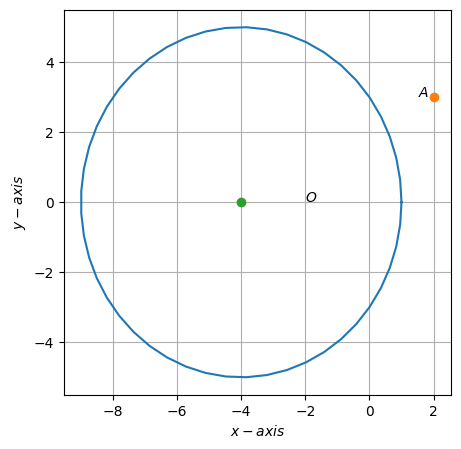
\includegraphics[width=\columnwidth]{chapters/11/11/1/13/fig/11.11.1.13.png}
    \caption{}
    \label{fig:11.11.1.13}
\end{figure}



\end{enumerate}
